% begin module sequence-squeeze-theorem
\begin{frame}
The Squeeze Theorem also works for sequences:
\begin{theorem}[The Squeeze Theorem for Sequences]
If $a_n\leq b_n\leq c_n$ for $n \geq n_0$ and $\lim_{n\to\infty} a_n = L = \lim_{n\to\infty}c_n$, then $\lim_{n\to\infty}b_n=L$.
\end{theorem}
\begin{center}
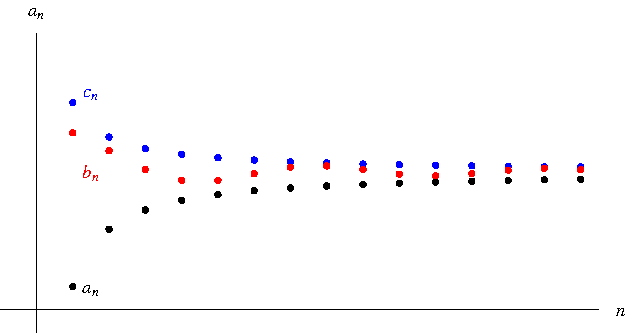
\includegraphics[width=8cm]{sequences/pictures/12-01-squeeze.pdf}%
\end{center}
\uncover<2->{%
%Here is a corollary to the Squeeze Theorem for sequences:
\begin{corollary}
If $\lim_{n\to\infty} |a_n| = 0$, then $\lim_{n\to\infty}a_n = 0$.
\end{corollary}
}%
\end{frame}
% end module sequence-squeeze-theorem
